\documentclass[catalan]{beamer}

\usepackage[utf8]{inputenc}
\usepackage[catalan]{babel}

\title{Plataforma eMovie: Xarxa social de pel·lícules}
\author{Roger Llopart Pla}
\date{\today}
\usetheme{Frankfurt}
\usecolortheme{beaver}

\begin{document}

\frame{\titlepage}

\section{Introducció}

\subsection{El problema}
\begin{frame}
\frametitle{El problema}
Actualment, a la web, hi ha massa contingut per a l'usuari que no està buscant rés concret.
\end{frame}

\subsection{La solució}
\begin{frame}
\frametitle{La solució}
{\Large{\bf Recomanar} a l'usuari únicament el contingut que li {\bf podria interessar}}.
\end{frame}

\section{Estat de l'art}

\subsection{Recomanadors}
\begin{frame}
\frametitle{Recomanadors}
\begin{center}
Tres categories de recomanadors diferents.
\end{center}
\vfill
\begin{columns}[c]
\column{.3\textwidth}
\textbf<2>{Recomanadors col·laboratius}
\column{.3\textwidth}
\textbf<3>{Recomanadors basats en contingut}
\column{.3\textwidth}
\textbf<4>{Recomanadors híbrids}
\end{columns}
\end{frame}

\subsection{Webs amb recomanació}

\begin{frame}
\frametitle{Webs amb recomanació: Netflix}
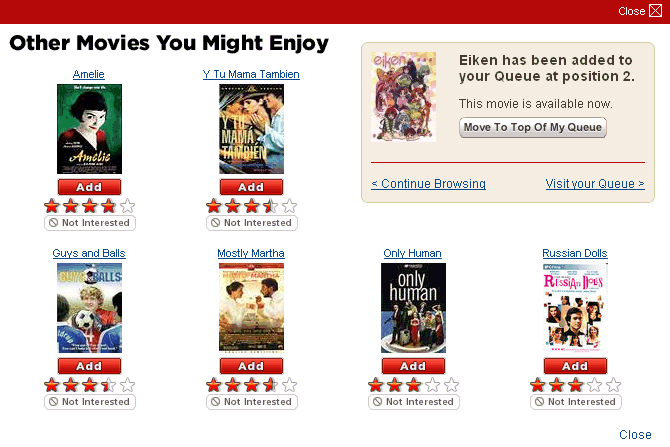
\includegraphics[width=\textwidth]{figs/netflix-recommendations}
\end{frame}

\begin{frame}
\frametitle{Webs amb recomanació: Movielens}
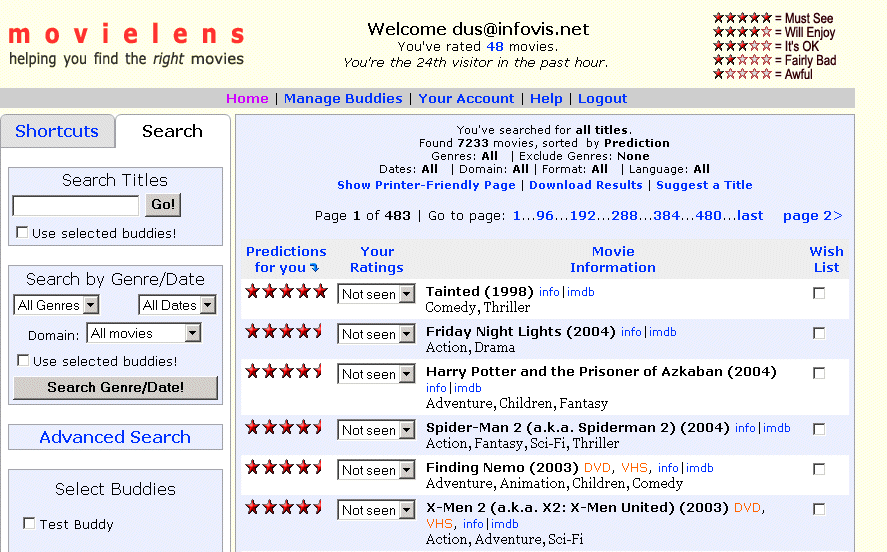
\includegraphics[width=\textwidth]{figs/movielens-recommendations}
\end{frame}

\begin{frame}
\frametitle{Webs amb recomanació: Rotten Tomatoes}
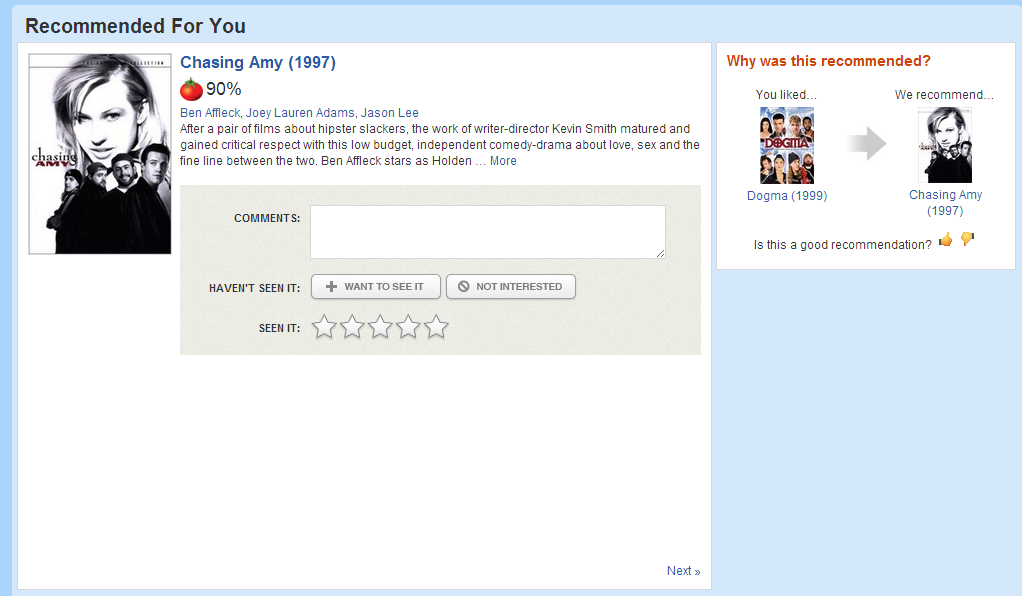
\includegraphics[width=\textwidth]{figs/rotten-tomatoes-recommendations}
\end{frame}

\begin{frame}
\frametitle{Webs amb recomanació: IMDb}
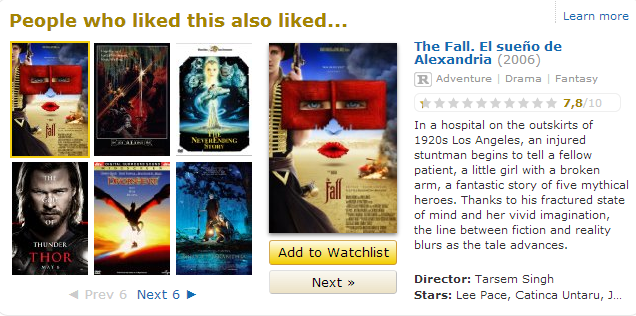
\includegraphics[width=\textwidth]{figs/imdb-recommendations}
\end{frame}

\section{Plataforma web}

\begin{frame}
\frametitle{Plataforma web}
Web desenvolupada amb PHP i MySQL.
\end{frame}

\subsection{Imatges de la web}
\begin{frame}
\frametitle{Index}
\begin{center}

\includegraphics[width=.7\textwidth]{figs/homepage}
\end{center}
\end{frame}

\begin{frame}
\frametitle{Resultats de cerca}
\begin{center}
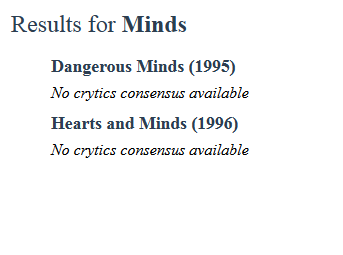
\includegraphics[width=.6\textwidth]{figs/resultats-busqueda}
\end{center}
\end{frame}

\begin{frame}
\frametitle{Fitxa de pel·lícula}
\begin{center}
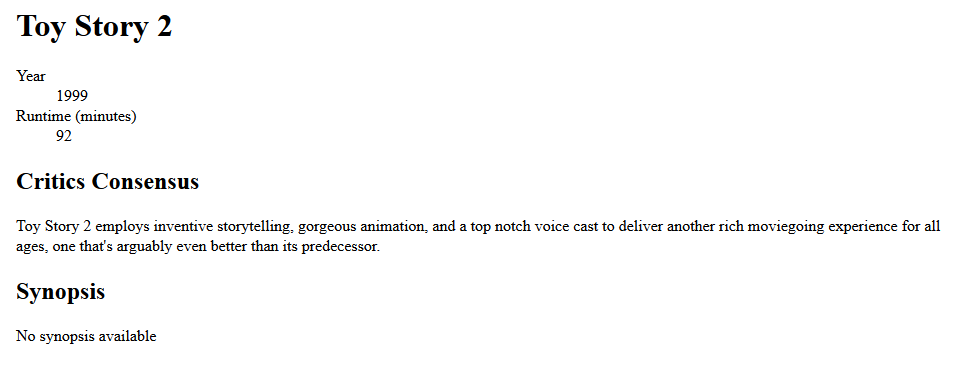
\includegraphics[width=\textwidth]{figs/film}
\end{center}
\end{frame}

\begin{frame}
\frametitle{Llistat de recomanacions}
\begin{center}
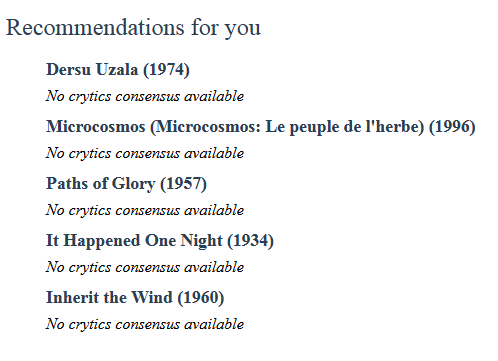
\includegraphics[width=.6\textwidth]{figs/recommendation}
\end{center}
\end{frame}


\section{Recomanadors}

\subsection{Implementació}
\begin{frame}
\frametitle{Implementació}
Implementació realitzada amb Mahout.
\end{frame}

\subsection{Recomanadors utilitzats}
\begin{frame}
\frametitle{Recomanador per veïnatge}
Fa servir la nota d'altres usuaris que hagin vist la pel·lícula tenint en compte quan semblants són respecte a l'usuari actual.
\end{frame}

\begin{frame}
\frametitle{Slope-One}
\begin{center}
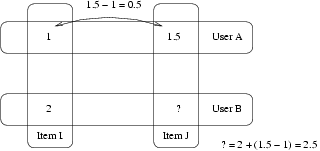
\includegraphics{figs/slope-one}
\end{center}
\end{frame}

\begin{frame}
\frametitle{Descomposició en Valors Singulars}
\begin{center}
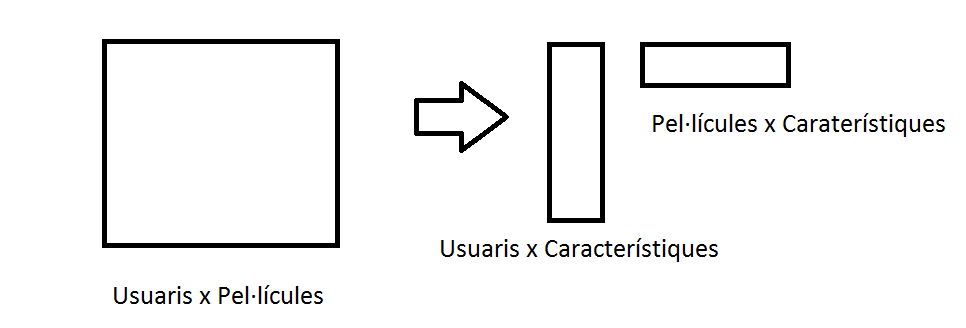
\includegraphics[width=\textwidth]{figs/svd}
\end{center}
\end{frame}

\subsection{Resultats}
\begin{frame}
\frametitle{Resultats}
S'ha avaluat el RMSE i la velocitat de resposta.
\end{frame}

\begin{frame}
\frametitle{Resultats}
\begin{center}
\begin{tabular}{|c|c|c|c|}\hline
		& Veïnatge	& Slope-One	& SVD 		\\ \hline
RMSE		& 1.0044	& 0.9193	& \textbf{0.9158}	\\
Velocitat	& 907.1	& 125.7	& \textbf{0.926}	\\ \hline
\end{tabular}
\end{center}
\end{frame}

\section{Conclusions}

\begin{frame}
\frametitle{Conclusions}

SVD dona bons resultats ja que abstrau més les puntuacions dels usuaris.

Té una bona velocitat de resposta ja que el còmput pesat es realitza durant l'entrenament.
\end{frame}

\begin{frame}
\frametitle{Possibles ampliacions}

Es podrien provar altres sistemes de recomanació, o combinació de varis.

També es podrien realitzar millores d'usabilitat i gràfiques a la web, i afegir funcionalitats adicionals.

\end{frame}

\frame{\titlepage}

\end{document}